\chapter{Ergebnisse}
\label{cpt:Ergebnisse}

Hier werden die eigenen Ergebnisse dargestellt. Die Eigenleistung sollte im Fokus stehen und somit auch den größten Teil der Arbeit ausmachen. 

Die Ergebnispräsentation kann durch graphische Darstellungen häufig gut unterstützt werden (vgl. \autoref{fig:Vgl_Exp_1_2}).
Besonders schön ist es dabei, wenn in der Graphik die gleiche Schriftart Verwendung findet wie sie im Text verwendet wird. Ebenfalls für einen besonders sauberen optischen Eindruck sorgen Vektorgrafiken. Gerade in den gedruckten Exemplaren fügen sich diese besser in das hochauflösende Schriftbild der Texte ein. Bei der Erstellung von Graphiken mit Python ist dies durch die Verwendung von \LaTeX -rendering möglich. Der Quelltext für \autoref{fig:Vgl_Exp_1_2} befindet sich in \autoref{Quelltext_A}. 

\begin{figure}[H]
	\centering
	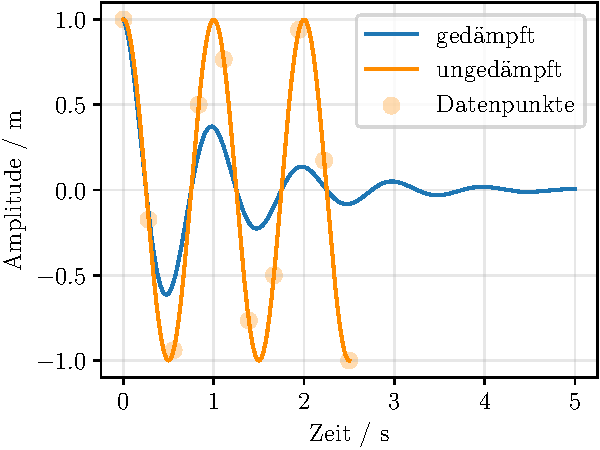
\includegraphics[scale=1]{/Schwingungen.pdf}
	\caption[Darstellung verschiedener Kosinunsschwingungen]{Darstellung einer gedämpften und einer ungedämpften Kosinusschwingung}
	\label{fig:Vgl_Exp_1_2}
\end{figure}

Es kann sinnvoll oder sogar notwendig sein, dass Daten geglättet oder zum Beispiel aufgrund physikalischer Zusammenhänge bestimmte Funktionen angenommen werden. Dabei ist es wichtig dem Betrachter der Graphik nicht zu suggerieren, dass die bearbeitete Darstellung den Messwerten entspricht. Um dies zu vermeiden sollten die tatsächlichen Datenpunkte mit dargestellt werden, wie in \autoref{fig:Vgl_Exp_1_2} am Beispiel der ungedämpften Schwingung dargestellt. Ist die Punktdichte sehr hoch und die Daten wurden nicht bearbeitet, ist dies nicht erforderlich, da es keinen informativen Mehrwert bietet.\\ 

Lässt sich die Unsicherheit der Daten angeben kann diese Beispielsweise durch graue Einfärbungen in die Graphik integriert werden und bietet so einen schnellen Überblick (vgl. \autoref{fig:Unsicherheit}), der Quelltext befindet sich in \autoref{Quelltext_B}. 

\begin{figure}[H]
	\centering
	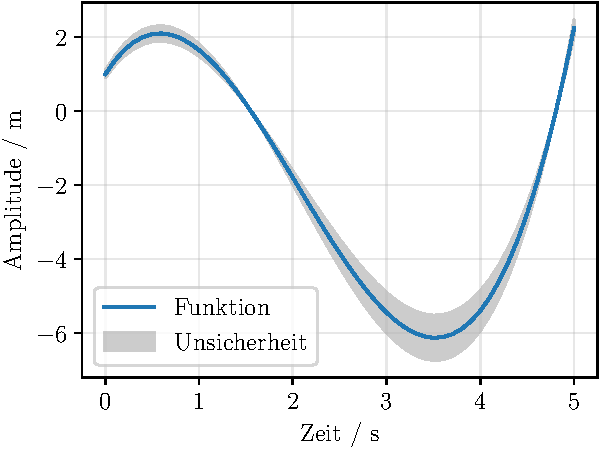
\includegraphics[scale=1]{/Fkt_mit_Unsicherheit.pdf}
	\caption{Darstellung einer Funktion mit Angabe des Unsicherheitsbereiches}
	\label{fig:Unsicherheit}
\end{figure}

Neben den bereits vorgestellten Graphen können auch andere Darstellungsformen Verwendung finden. In \autoref{fig:Boxplot} sind Beispielhaft Boxplots dargestellt. Die Darstellungsform sollte sorgsam gewählt werden um den Betrachter beim erfassen der relevanten Informationen so gut wie möglich zu unterstützen.

\begin{figure}[H]
	\centering
	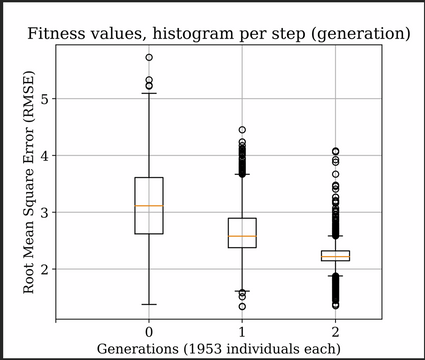
\includegraphics[scale=.5]{/Boxplot.png}
	\caption{Darstellung mehrerer Boxplots}
	\label{fig:Boxplot}
\end{figure}

Auch Tabellen können einen guten Überblick über die Arbeit ermöglichen (vgl. \autoref{tab:example}). Diese können auch mit verschiedenen \href{https://www.tablesgenerator.com/}{Online Tools} vorformatiert werden , dies ist insbesondere dann sinnvoll, wenn die Tabellenköpfe etwas verschachtelter sind.

\begin{table}[H]
	\caption{Das ist ein Beispiel für eine Tabelle}
	\label{tab:example}
	\begin{tabular}{|l|l|l|l|l|}
		\hline
		\multicolumn{1}{|c|}{\multirow{2}{*}{\textbf{NR.}}} & \multicolumn{2}{c|}{\textbf{Kategorie 1}}               & \multicolumn{2}{c|}{\textbf{Kategorie 2}}               \\ \cline{2-5} 
		\multicolumn{1}{|c|}{}                              & \textit{Unterkategorie 11} & \textit{Unterkategorie 12} & \textit{Unterkategorie 21} & \textit{Unterkategorie 22} \\ \hline
		1	&                            &                            &                            &                            \\ \hline
		2	&                            &                            &                            &                            \\ \hline
	\end{tabular}
\end{table}

Den Abschluss des Kapitels der Ergebnisse sollte die Einordnung der Ergebnisse in den wissenschaftlichen Gesamtkontext bilden. 
